%%%%%%%%%%%%%%%%%%%%%%%%%%%%%%%%% Packages/Dokumentart %%%%%%%%%%%%%%%%%%%%%%%%%%%%%%%%%%%%%%%%%%%%%%%%%%%%%%%%%%%%%%%%%%%%%%%%%%%%%%%%%%%%%%%%%%%%%%%%%%%%%%%%%%%%%%%
\documentclass[ a4paper,	% Papierart
	%       10pt,		%
		11pt,		% Schriftgröße
	%	12pt,		%
		pdftex,		% PDF Umwandlung
	%	twoside		% 2-seitig
		] {report}	% Dokumenttyp Bericht

\usepackage[ngerman]{babel}	% Deutsches Sprachpaket/Silbentrennung etc.
%\usepackage[utf8]{inputenc}	% verwendeter Codec (für Umlaute)
\usepackage{graphicx}		% für Bilder
\usepackage{cite}		% für bestimmte Zitierfunktionen
\usepackage[footnote]{acronym}	% für Abkürzungen in Fußnote
\usepackage{caption}		% Um Bildunterschriften zu konfigurieren (mit, ohne erscheinen im Abkürzungsverzeichnis)
\usepackage{setspace}		% für Zeilenabstand
\usepackage{listings}
\usepackage{color}
 

 \definecolor{middlegray}{rgb}{0.5,0.5,0.5}
 \definecolor{lightgray}{rgb}{0.8,0.8,0.8}
 \definecolor{orange}{rgb}{0.8,0.3,0.3}
 \definecolor{yac}{rgb}{0.6,0.6,0.1}
 \lstset{
   basicstyle=\scriptsize\ttfamily,
   keywordstyle=\bfseries\ttfamily\color{orange},
   stringstyle=\color{green}\ttfamily,
   commentstyle=\color{middlegray}\ttfamily,
   emph={square}, 
   emphstyle=\color{blue}\texttt,
   emph={[2]root,base},
   emphstyle={[2]\color{yac}\texttt},
   showstringspaces=false,
   flexiblecolumns=false,
   tabsize=2,
   numbers=left,
   numberstyle=\tiny,
   numberblanklines=false,
   stepnumber=1,
   numbersep=10pt,
   xleftmargin=15pt
 }




\onehalfspacing			% ab hier Zeilenabstand 1,5


%%%%%%%%%%%%%%%%%%%%%%%%%%%%%%%% Kopfzeile %%%%%%%%%%%%%%%%%%%%%%%%%%%%%%%%%%%%%%%%%%%%%%%%%%%%%%%%%%%%%%%%%%%%%%%%%%%%%%%%%%%%%%%%%%%%%%%%%%%%%%%%%%%%%%%%%%%%%%%%%%
\usepackage[automark]{scrpage2}			% Package für Kopfzeile	
\pagestyle{scrheadings} 			% Pagestyle
\automark[section]{chapter} 			% für Anzeigen des Unterkapitels (Standard Überkapitel)
\clearscrheadfoot \ihead{\headmark}		% ihead links, ohead rechts, chead mitte
\setheadsepline{0.4pt}				% Linie unter Kopfzeile
\cfoot[\pagemark]{\pagemark}			% Mitte Fußzeile Seitenzahl (selbe wie mit head (i,o,c))

%%%%%%%%%%%%%%%%%%%%%%%%%%%%%%%%%% Abkürzungen %%%%%%%%%%%%%%%%%%%%%%%%%%%%%%%%%%%%%%%%%%%%%%%%%%%%%%%%%%%%%%%%%%%%%%%%%%%%%%%%%%%%%%%%%%%%%%%%%%%%%%%%%%%%%%%%%%%%%%%
% Persöhnlich

\newcommand{\Was}{ PIC16F84A}

\newcommand{\Titel}{Simulator für den Mikrocontroller }


\begin{document}   %%%%%%%%%%%%%%%%%%%%%%%%%%%%%%%%%%%%%%%%%%%%%%%%%%%%%%%%%%%%%%%%%%%%%%%%%%%%%%%%%%%%%%%%%%%%%%%%%%%%%%%%%%%%%%%%%%%%%%%%%%%%%%%%%%%%%%%%%%%%%%%%%%%%

%%%%%%%%%%%%%%%%%%%%%%%%%%%%%%%%%% Titelseite %%%%%%%%%%%%%%%%%%%%%%%%%%%%%%%%%%%%%%%%%%%%%%%%%%%%%%%%%%%%%%%%%%%%%%%%%%%%%%%%%%%%%%%%%%%%%%%%%%%%%%%%%%%%%%%%%%%%%%%%%
\begin{singlespace}							% Zeilenabstand für Titelseite verringern
\begin{titlepage}
\begin{center}								% Referenzpunkt Seitenmitte
\vspace*{-2cm}								% 2 cm nach Links Platz lassen
\hfill
\includegraphics[width=4cm]{Bilder/dhbw-logo}\\[2cm] % Firmenlogo platzieren

{\Huge \Titel}\\[0.5cm]							% \Huge, \Large, \large sind versch. Schriftgrößen \bfseries ist Fett gedruckt
{\Huge \Was}\\[1cm]						% [] Inhalt ist Abstand zur nächsten Zeile

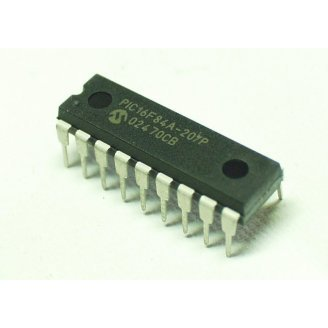
\includegraphics[width=4cm]{Bilder/Microcontroller.jpg}\\[2cm]

{\large von\\[0.5cm]
{\large Michael Stahlberger und Julian Kühn}\\[0.5cm]

{\large Studiengang Informationstechnik \\
an der Dualen Hochschule Karlsruhe}\\[0.5cm]}

\vfill									% ermöglicht es unterhalb der Seitengrenze zu schreiben
\end{center}								% Referenzpunkt Mitte beenden

							% Tabelle abschließen
\end{titlepage}
\end{singlespace}								% Titelseite abschließen
%%%%%%%%%%%%%%%%%%%%%%%%%%%%%%%%%%%%%%%%%%%%%%%%%%%%%%%%%%%%%%%%%%%%%%%%%%%%%%%%%%%%%%%%%%%%%%%%%%%%%%%%%%%%%%%%%%%%%%%%%%%%%%%%%%%%%%%%%%%%%%%%%%%%%%%%%%%%%%%%%%%%%%%%
 %%%%%%%%%%%%%%%%%%%%%%%%%%%%%%%%%%%%%%%%%%%%%%%%%%%%%%%%%%%%%%%%%%%%%%%%%%%%%%%%%%%%%%%%%%%%%%%%%%%%%%%%%%%%%%%%%%%%%%%%%%%%%%%%%%%%%%%%%%%%%%%%%%%%%%%%%%


%%%%%%%%%%%%%%%%%%%%%%%%%%%%%%%%%% Verzeichnisse %%%%%%%%%%%%%%%%%%%%%%%%%%%%%%%%%%%%%%%%%%%%%%%%%%%%%%%%%%%%%%%%%%%%%%%%%%%%%%%%%%%%%%%%%%%%%%%%%%%%%%%%%%%%%%%%%%%%%%%%


\begin{singlespace}			 % Zeilenabstand für Verzeichnisse 1	
\tableofcontents 			 % Inhaltsverzeichnis
\listoffigures	 			 % Abbildungsverzeichnis
\end{singlespace}	 		 % Zeilenabstand wieder ausstellen
%\listofequations			 % Formelverzeichnis
\lstlistoflistings
			 % Listenverzeichnis

\newpage %%%%%%%%%%%%%%%%%%%%%%%%%%%%%%%%%%%%%%%%%%%%%%%%%%%%%%%%%%%%%%%%%%%%%%%%%%%%%%%%%%%%%%%%%%%%%%%%%%%%%%%%%%%%%%%%%%%%%%%%%%%%%%%%%%%%%%%%%%%%%%%%%%%%%%%%%%%%%%%%%

%%%%%%%%%%%%%%%%%%%%%%%%%%%%%%%%%% Kapitel einbinden %%%%%%%%%%%%%%%%%%%%%%%%%%%%%%%%%%%%%%%%%%%%%%%%%%%%%%%%%%%%%%%%%%%%%%%%%%%%%%%%%%%%%%%%%%%%%%%%%%%%%%%%%%%%%%%%%%%%%
\chapter{Einleitung}			% Kapitelname

Die Zielsetzung des Projektes ist es einen Simulator f\"ur einen PIC16F84A Mikrocontroller zu schreiben. Dabei sollen verschieden Debug-Funktionen ebenfalls implementiert werden. Es soll M\"oglich sein ein korrekt geschriebenes Programm zu testen und zu debuggen.

\section{Was ist ein Simulator?}

Eine Simulation ist ein möglichst realitätsnahes Nachbilden von Geschehen der Wirklichkeit. Aus Sicherheits- und Kostengründen ist es für fast alle Anwendungsgebieten notwendig. Die gewonnenen Erkenntnisse können nach einer Simulation auf die Realität übertragen werden. Eine Simulation findet meistens nicht in Echtzeit statt (wie z.B. bei einer Emulation) sondern wird zu analytischen Zwecken langsamer als in der Realität nachgebildet.			% Einbinden der Unterkapitel
\section{Vor- und Nachteile eines Simulators}

\textbf{Vorteile:}
Durch eine Simulation k\"onnen Versuche die unter gef\"ahrlichen Umst\"anden stattfinden m\"ussen sicher nachgestellt werden (z.B. Crash-Simulationen mit Autos und Crash-Test-Dummys).
Aber auch Versuche die aus Kostengr\"unden in der Realit\"at oftmals schwierig nachzustellen sind k\"onnen durch Simulationen begrenzt ersetzt werden.
Durch den verlangsamten Ablauf einer Simulation sind au\ss erdem Fehler oder Ergebnisse leichter nachzuvollziehen als in der Wirklichkeit.
Im Falle des Mikrocontrollers k\"onnen Programme vor ihrem praktischen Einsatz getestet und debuggt werden um so m\"ogliche Fehler im Praxiseinsatz fr\"uhzeitig zu erkennen und auszubessern.\\
\\
\textbf{Nachteile:}
Eine Simulation ist meist durch begrenzte Ressourcen eingeschr\"ankt. Sei es die Rechenleistung einer Computersimulation oder Geld und Zeit die f\"ur eine Simulation eingesetzt werden m\"ussen. Oftmals wird deswegen nur ein vereinfachtes Modell der Wirklichkeit eingesetzt. Durch diese Vereinfachung kann es zu ungenauen Messergebnisse oder Situationen kommen die in der Realit\"at vielleicht gar nicht vorkommen.
F\"ur den PIC16-Simulatior ist es wichtig m\"oglichst fehlerfrei und genau zu arbeiten da Fehler innerhalb der Simulation auf falsche R\"uckschl\"usse auf das f\"ur den Mikrocontroller entwickelte Programm f\"uhren k\"onnte. Auch zu bedenken ist es das die Laufzeit in der Simulation nicht der Realzeit entspricht und somit das Programm in der Realit\"at schneller sein w\"urde.			% Einbinden der Unterkapitel
\section{Mikrocontroller PIC16F84A}

Ein Mikrocontroller ist eine Art Mikrorechnersystem, bei welchem neben ROM und RAM auch Peripherieeinheiten wie Schnittstellen, Timer und Bussysteme auf einem einzigen Chip integriert sind.
Die Hauptanwendungsgebiete sind die Steuerungs-, Mess- und Regelungstechnik, sowie die Kommunikationstechnik und die Bildverarbeitung. Mikrocontroller sind in der Regel in Embedded Systems, in die Anwendung eingebettete Systeme, und somit in der Regel von au\ss en nicht sichtbar. Ebenso verf\"ugen sie, im Gegensatz zum PC, nicht \"uber eine direkte Bedien- und Prorgrammierschnittstelle zum Benutzer. Sie werden in der Regel einmal programmiert und installiert.

Der PIC16F84 Mikrocontroller ist ein 8 Bit Mikrocontroller mit RISC-Architektur (Reduced-Instruction-Set-Computing). Es wird also auf komplexe Befehle verzichtet und mit jedem Befehl kann auf jedes Register zugegriffen werden. Der Mikrocontroller besitzt durch die eingesetzte Harvard-Architektur bis zu 14 Bit gro\ss e Befehle w\"ahrend die Gr\"o\ss e des separaten Datenbusses nur 8 Bit betr\"agt.

\begin{figure}[htb]
\centering
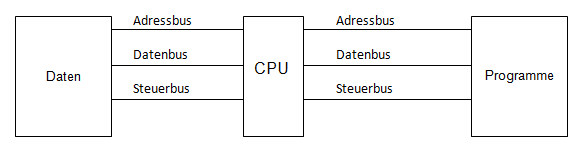
\includegraphics{Bilder/Harvard}
\caption{Harvard-Architektur}
\end{figure}

\newpage
Durch die Architektur ben\"otigen fast alle Anweisungen nur einen Instruction Cycle (Abarbeitung eines Maschinenbefehls).
Der PIC16 besitzt einen Stack mit Speicherplatz f\"ur 8 Adressen sowie 2 externe und 2 interne Interrupt Quellen. Dar\"uber hinaus besitzt der Pic16F ein gro\ss es Register, welches in zwei B\"anke unterteilt ist. Das Umschalten der B\"anke erfolgt im Programmcode. Die Speicherbereiche k\"onnen auch direkt \"uber ihre Registeradresse angesprochen werden.
			% Einbinden der Unterkapitel
\newpage

\chapter{Tools}			% Kapitelname


\section{Entwicklungsumgebung Eclipse}

Eclipse ist eine freie Entwicklungsumgebung welche ursrp�nglich f�r die Sprache Java entwickelt wurde. Mittlerweile gibt es Eclipse Plug-ins f�r weitere Programmiersprachen wie C, C++ oder Pearl.
Wie die meisten Entwicklungsumgebungen bietet Eclipse eine Vielzahl, dem Entwickler n�tzlicher, Funktionen. Dazu geh�ren das Debuggen des Programmcodes, automatische Erstellen von Get- und Set- Methoden sowie automatische Codevervollst�ndigung. �ber automatische Kontexthilfe liefert Eclipse Vorschl�ge um Fehler zu beheben.
Eclipse kann leicht durch den Eclipse Marketplace mit verschienden Plug-Ins erweitert werden. F�r die Verbindung von Eclipse mit dem eingesetzten Versionsverwaltungs System Git wurde das Plug-In EGit verwendet.


\begin{figure}[h]
\centering
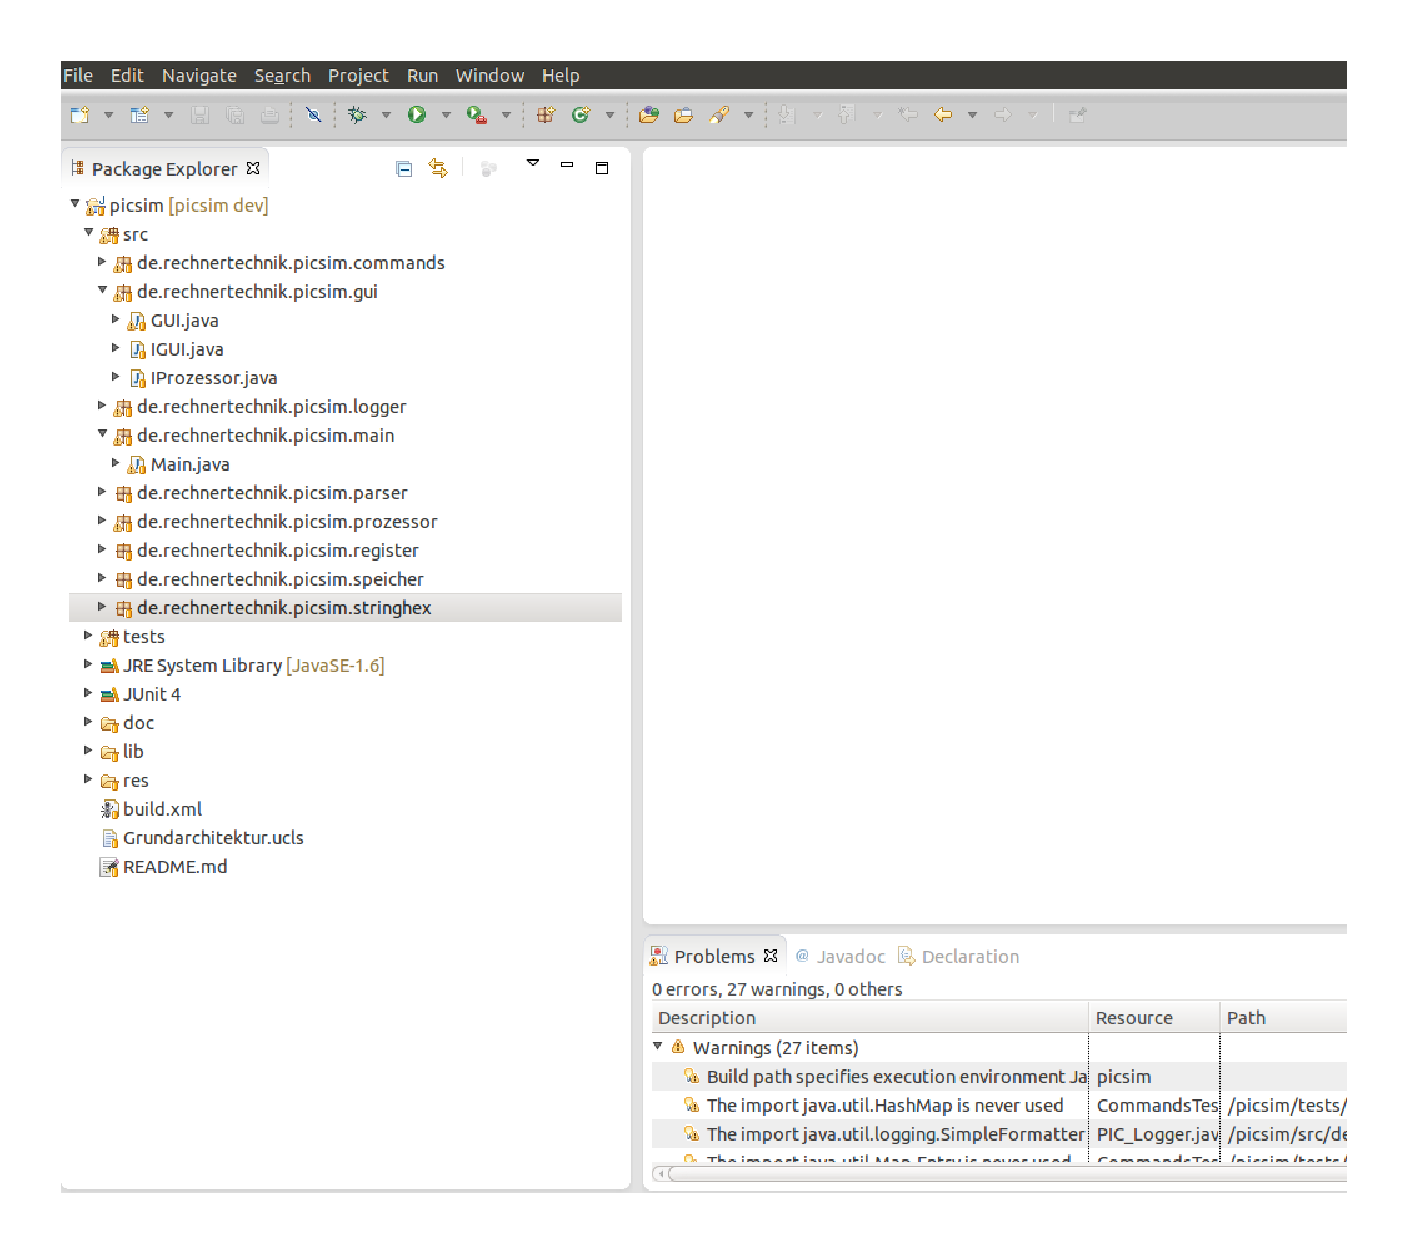
\includegraphics[scale=0.25]{Bilder/Eclipse.pdf}
\caption{Eclipse}
\end{figure}			% Einbinden der Unterkapitel
\newpage
\section{Versionsverwaltung Git}
Git ist eine freie Software zur verteilten Versionsverwaltung von Dateien, die urspr\"unglich f\"ur die Quellcode-Verwaltung des Linux-Kernels entwickelt wurde. Git speichert die Daten nicht auf einen zentralen Server sondern bei jedem User zun\"achst lokal in einem s.g. Repository. So besitzt jeder User den gesamten Code so wie die Versionsgeschichte zun\"achst auf seinem eigenen PC. Ein Remote Repository ist ein Repository das nicht lokal auf dem eigenen Rechner verf\"ugbar ist sondern zentral auf einem Server ausgelagert wird. \"uber einen Push Befehl kann das Remote Repository mit dem lokalem Repository \"uberschrieben werden. Wird ein Fetch Befehl ausgef\"uhrt wird dass Remote Repository mit dem lokalem Repository verglichen und zusammengef\"uhrt (merge Befehl) werden. Im Projekt wurde GitHub, ein webbasierter Hosting-Dienst f\"ur Software-Entwicklungsprojekte verwendet.


\begin{figure}[h]

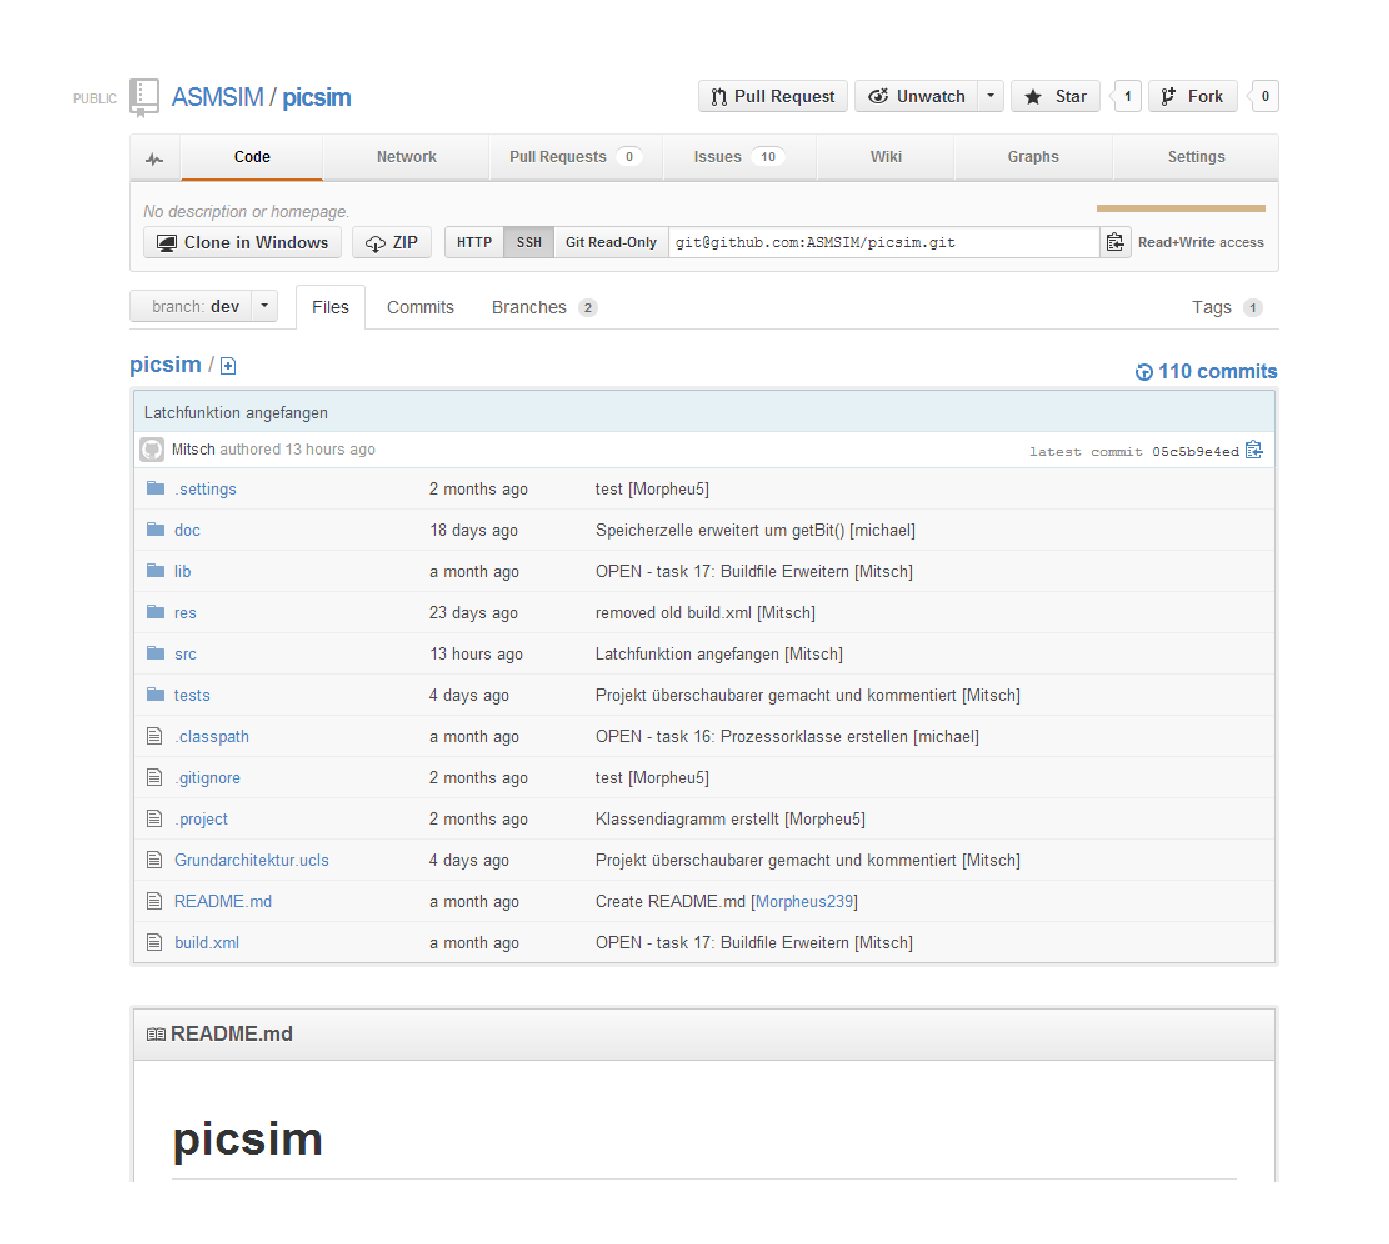
\includegraphics[scale=0.55]{Bilder/Github.pdf}
\caption{Github}
\end{figure}
			% Einbinden der Unterkapitel

\newpage

\chapter{Programmstruktur und Aufbau}			% Kapitelname

\section{Benutzeroberfl\"ache}

Beim Starten der Applikation \"offnet sich das User Interface des Simulators auf dem die Funktionen des PICs nachvollzogen werden k\"onnen.

\begin{figure}[h]
\centering
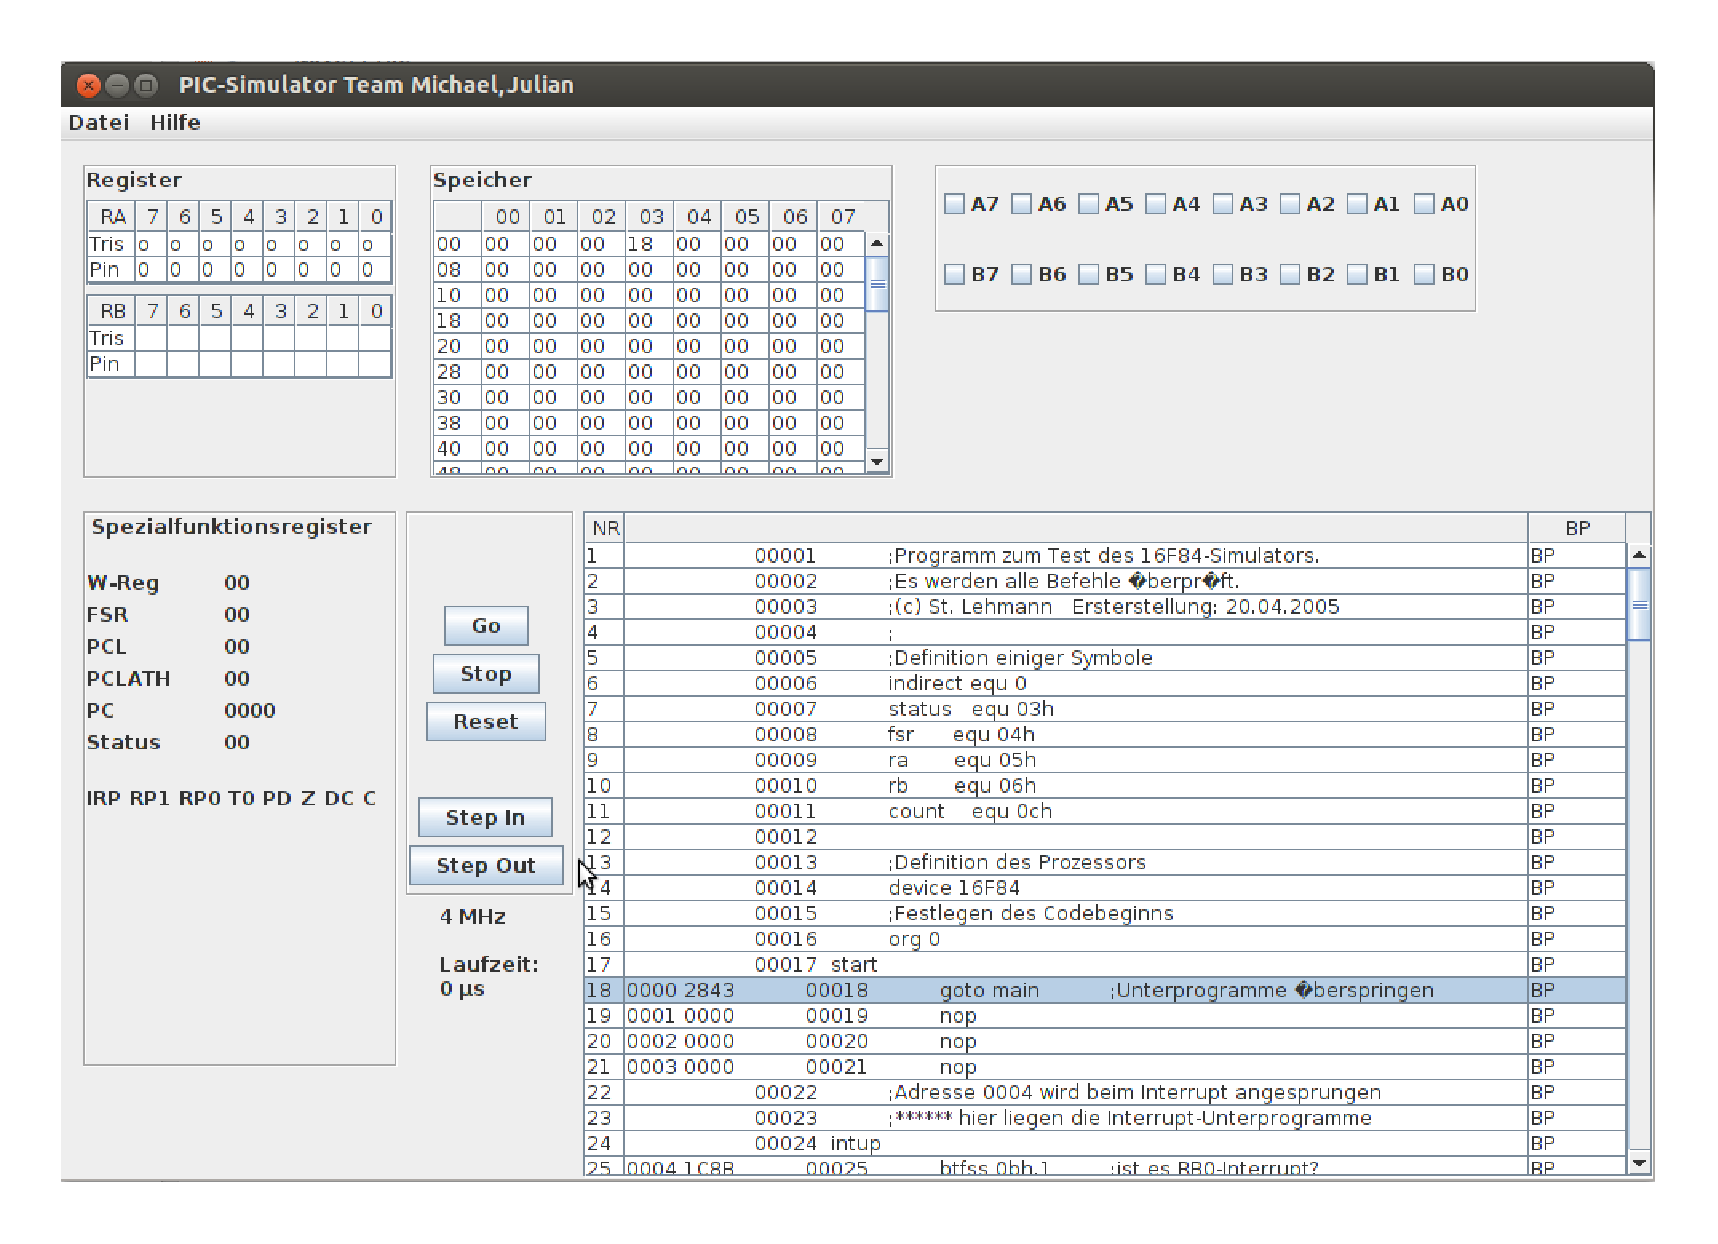
\includegraphics[scale=0.4]{Bilder/GUI.pdf}
\caption{GUI}
\end{figure}
\newpage

\noindent \"Uber „Datei“ und „Datei \"offnen“ lassen sich Quellcode-Dateien \"offnen. In die Dateiauswahl ist ein Dateifilter integriert der ausschließlich .LST-Dateien anzeigt.

\begin{figure}[h]
\centering
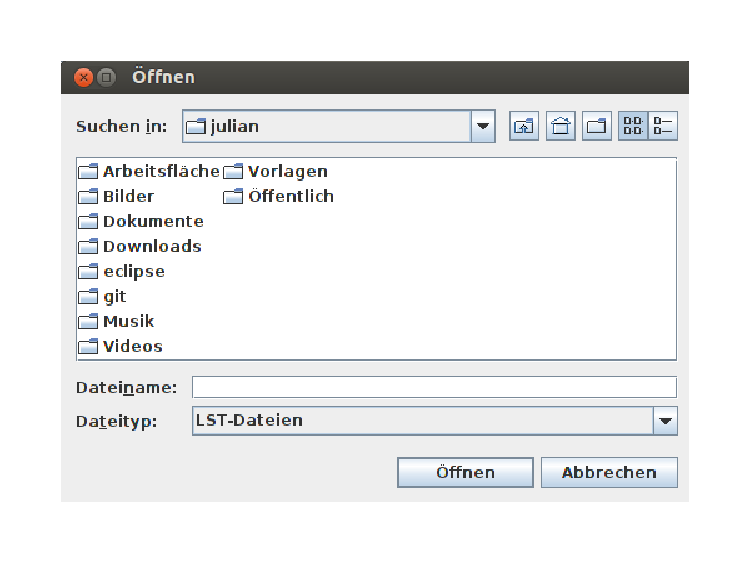
\includegraphics[scale=0.7]{Bilder/Offnen.pdf}
\caption{Datei \"offnen}
\end{figure}

\noindent Mit den Buttons \glqq Step-In\grqq , \glqq Step-Out\grqq , \glqq Go\grqq , \glqq Stop\grqq  und \glqq Reset\grqq  l\"asst sich der Simulationsablauf steuern. Mit Step-In und Step-Out l\"asst sich jeweils nur ein Programmschritt ausf\"uhren, mit Go wird das Programm komplett abgearbeitet. Mit Stop stoppt der Simulationsvorgang und mit Reset wird er komplett zur\"uckgesetzt.

\begin{figure}[h]
\centering
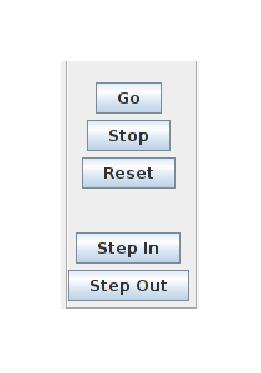
\includegraphics[scale=0.5]{Bilder/Buttons.pdf}
\caption{Kontroll-Buttons}
\end{figure}

Die Register werden in der linken oberen Ecke des User Interfaces angezeigt. Die werte des Spezialfunktionsregister wird darunter dargestellt. Die  Darstellung der Werte erfolgt im Hexadezimalsystem.

\begin{figure}[h]
\centering
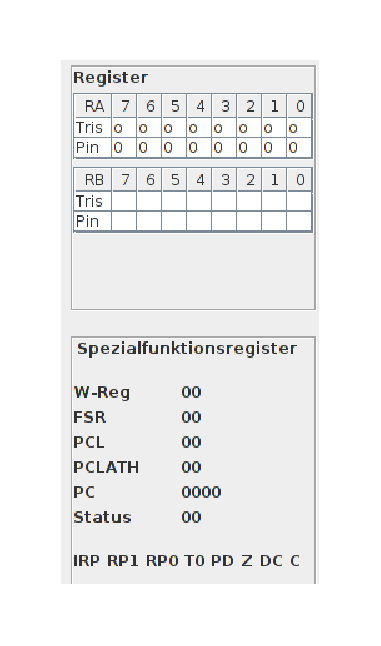
\includegraphics[scale=0.5]{Bilder/Register.pdf}
\caption{Register und Spezialfunktionsregister}
\end{figure}

Die Speicherinhalte werden in Form einer Tabelle am oberen Rand des User Interfaces dargestellt. Die Werte werden im Hexadezimalsystem wiedergegeben. 


\noindent In der rechten unteren Ecke wir der Quelltext des zu simulierenden Programmes angezeigt. Dieser wir wie beschrieben \"uber \glqq Datei \"offnen\grqq in die Tabelle geschrieben.

\begin{figure}[h]
\centering
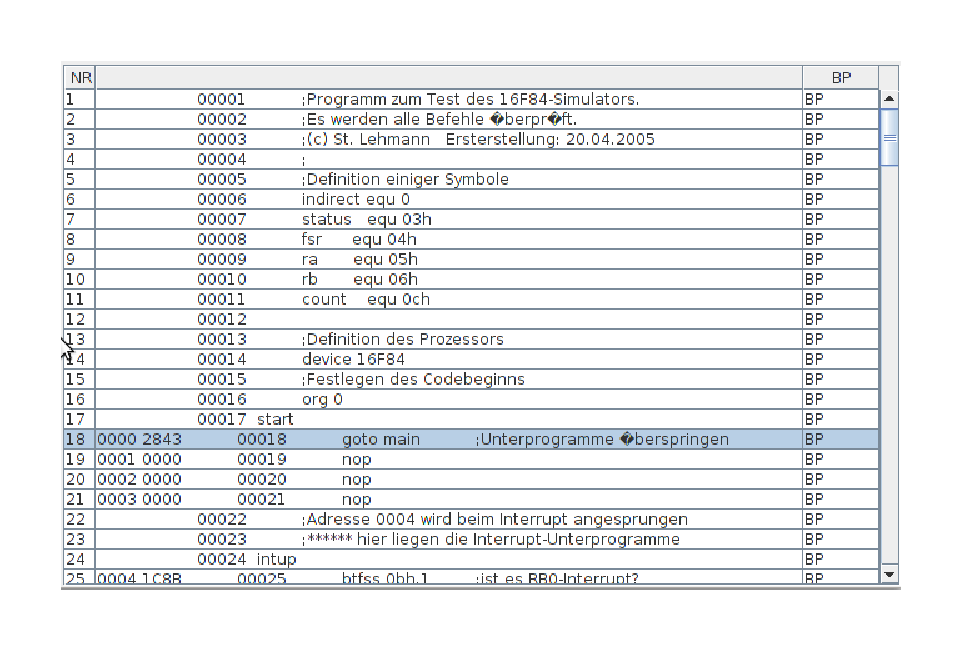
\includegraphics[scale=0.5]{Bilder/Text.pdf}
\caption{Textfeld f\"ur den Quelltext}
\end{figure}			% Einbinden der Unterkapitel
\section{Programmablauf}			% Einbinden der Unterkapitel
\newpage
\section{Beschreibung einiger Befehle}

\subsection{DECF}
In diese Beispiel wird das Ergebnis entweder in f oder in w gespeichert.

\begin{figure}[h]
\centering
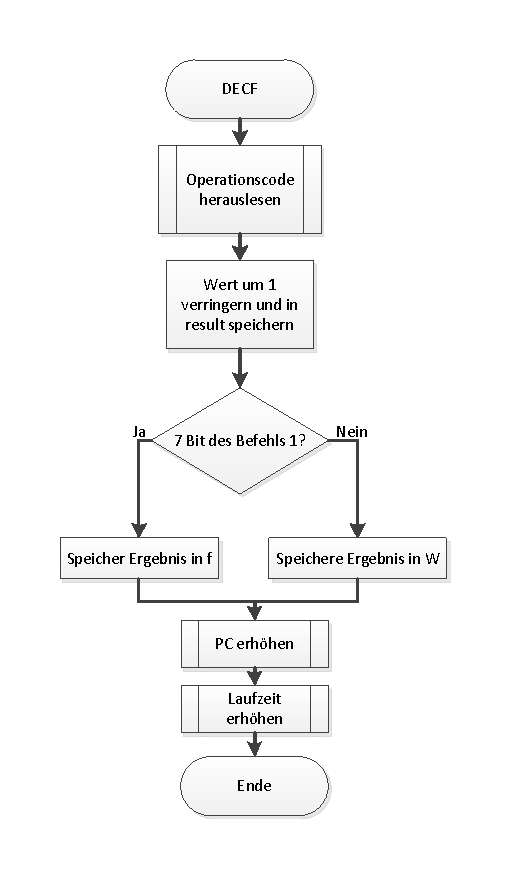
\includegraphics[scale=0.6]{Diag/DECF.pdf}
\end{figure}
\lstinputlisting[language=java]{Listings/DECF.java}

\newpage
\subsection{MOVF}


\begin{figure}[h]
\centering
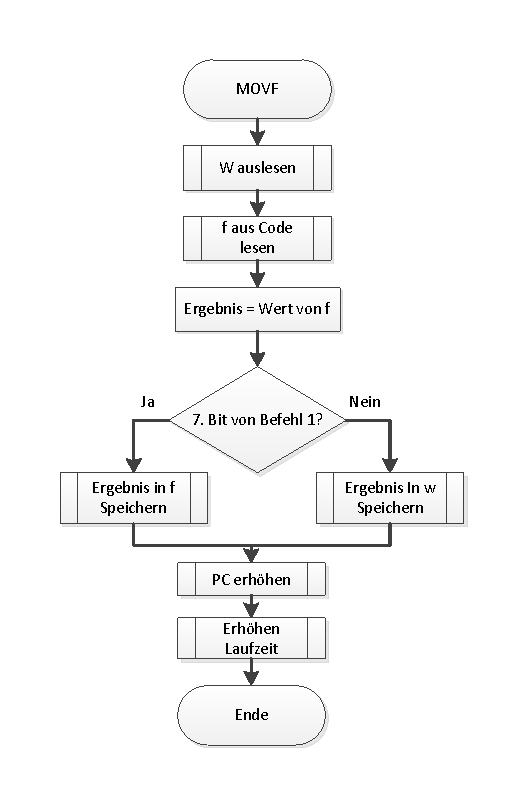
\includegraphics[scale=0.7]{Diag/MOVF.pdf}
\end{figure}
\lstinputlisting[language=java]{Listings/MOVF.java}
\newpage
\subsection{BTFSS}



\begin{figure}[h]
\centering
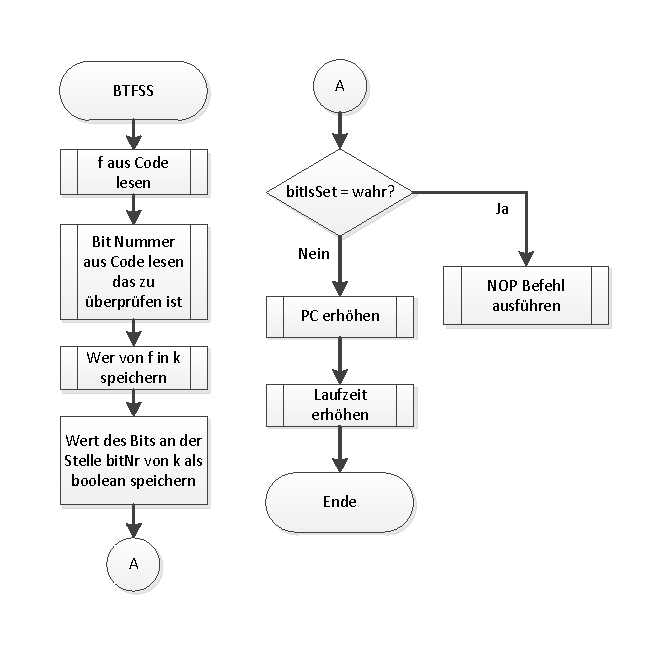
\includegraphics[scale=0.7]{Diag/BTFSS.pdf}
\end{figure}
\lstinputlisting[language=java]{Listings/BTFSS.java}
\newpage
\subsection{SUBLW}



\begin{figure}[h]
\centering
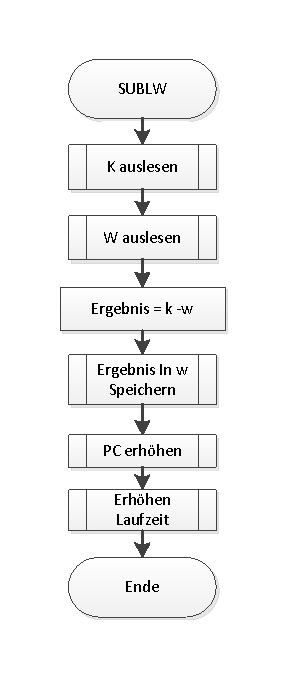
\includegraphics[scale=0.7]{Diag/SUBLW.pdf}
\end{figure}
\lstinputlisting[language=java]{Listings/SUBLW.java}
\newpage
\subsection{CALL}



\begin{figure}[h]
\centering
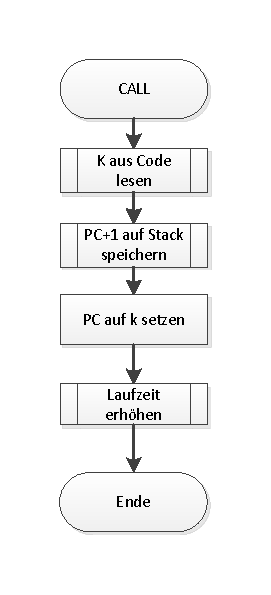
\includegraphics[scale=0.7]{Diag/CALL.pdf}
\end{figure}
\lstinputlisting[language=java]{Listings/CALL.java}	

\newpage
\section{Interrupt}
Bei einem Interrupt verl\"asst der PIC16F seine normale Routine und springt in eine Interruptroutine, die er abarbeitet um dann wieder an die Stelle des normalen Ablaufs zur\"uckzukehren.
\\
\noindent Im Simulator wird zwischen jedem Funktionsaufruf der einen Befehl beschreibt \"uberpr\"uft ob ein Interrupt stattfindet.
\\
\lstinputlisting[language=java]{Listings/Interrupt.java}
\noindent Bevor der Interrupt ausgef\"uhrt wird muss zuerst gepr\"uft werden ob das GIE (Global Interrupt enable), das INTE Bit im INTCON Register oder das T01E Bit f\"ur den Timer0 Interrupt gesetzt worden ist.
\\
\\Ist das INTE Bit gesetzt wird die Methode checkExternalInterrupt ausgef\"uhrt. In dieser Methode wird zun\"achst \"uberpr\"uft ob es sich um eine steigende oder fallende Flanke handelt (oldValue speichert immer den vorherigen Zustand von RB0). Nach der \"Uberpr\"ufung wird die Methode externerInteruptRB0 ausgef\"uhrt.
\\
\lstinputlisting[language=java]{Listings/InterruptRB0.java}
In dieser Methode  wird das Interrupt Flag gesetzt und die Methode InterruptHasOccured aufgerufen in der der eigentliche Interruptvorgang ausgef\"uhrt wird. Dort wird zun\"achst das GIE Bit auf 0 gesetzt, der Programm Counter auf dem Stack gespeichert und zum eigentlichen Interruptvektor gesprungen.
\\
\lstinputlisting[language=java]{Listings/InterruptOcc.java}
\newpage
\noindent F\"ur den Timer 0 Interrupt wird in der checkInterrupt Methode nach erfolgreicher \"Uberpr\"ufung checkTimer0Interrupt aufgerufen in der zun\"achst \"uberpr\"uft wird ob ein Timer 0 Interrupt stattgefunden hat. Daraufhin wird die Methode InterruptHasOccured aufgerufen wird (wie bei RB0). 
\lstinputlisting[language=java]{Listings/InterruptTime.java}
\\

\section{TRIS-Register}
Die TRIS-Register (TRI-State Enable) ist ein programmierbares 8 Bit Register welches einen Pin als Input oder Output konfiguriert. Jeder Port besitzt ein TRIS Register welches deren Pinzust\"ande beschreibt.
\\
\\Im Simulator wird bevor ein Port-Bit gesetzt wird zun\"achst sein TRIS-Status \"uberpr\"uft. Der gew\"unscht Pin wird nur ver\"andert wenn der richtige Zustand im TRIS Register steht.
\\
\lstinputlisting[language=java]{Listings/TRIS.java}


\section{Klassendiagramm}
\newpage

\chapter{Zusammenfassung}			% Kapitelname

\section{Umsetzung}
			% Einbinden der Unterkapitel
\section{Fazit}			% 
\newpage
%%%%%%%%%%%%%%%%%%%%%%%%%%%%%%%%%% Literaturverzeichnis %%%%%%%%%%%%%%%%%%%%%%%%%%%%%%%%%%%%%%%%%%%%%%%%%%%%%%%%%%%%%%%%%%%%%%%%%%%%%%%%%%%%%%%%%%%%%%%%%%%%%%%%%%%%%%%%%%
\addcontentsline{toc}{chapter}{Literaturverzeichnis}
\bibliographystyle{gerabbrv}				% Zitierformat (deutsch für Großschreibung) [Häufigkeit] im Text
\bibliography{Literaturverzeichnis}			% Pfad des Literaturverzeichnisses

\end{document}  %%%%%%%%%%%%%%%%%%%%%%%%%%%%%%%%%%%%%%%%%%%%%%%%%%%%%%%%%%%%%%%%%%%%%%%%%%%%%%%%%%%%%%%%%%%%%%%%%%%%%%%%%%%%%%%%%%%%%%%%%%%%%%%%%%%%%%%%%%%%%%%%%%%%%%%%%%

